%
% k-kruemmung.tex -- Krümmungstensor, Ricci, Einstein
%
% (c) 2017 Prof Dr Andreas Müller, Hochschule Rapperswil
%
\section{Krümmung
\label{skript:kruemmung:section:kruemmung}}

\begin{figure}
\centering
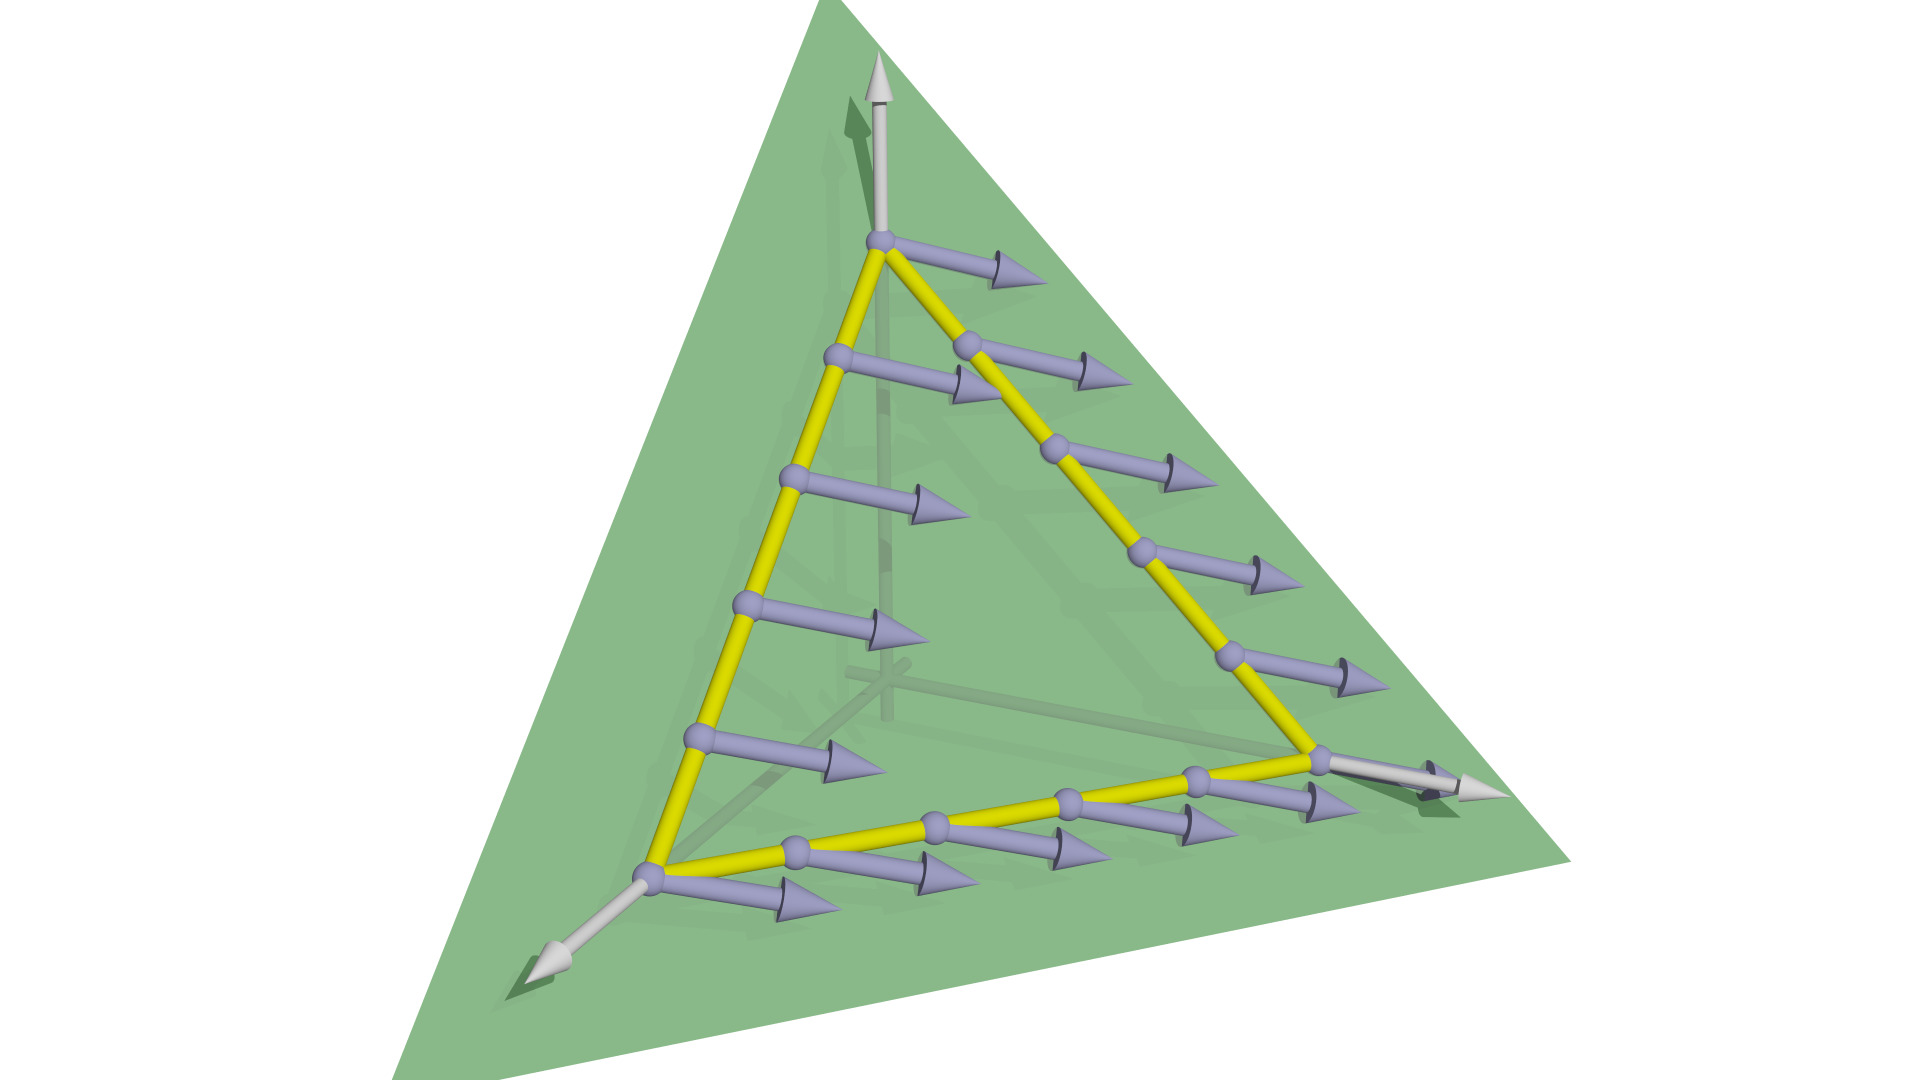
\includegraphics[width=\hsize]{chapters/3d/flach.jpg}
\caption{Beim Paralleltransport eines Vektors entlang einer Kurve in
einer Ebene dreht sich der Vektor nicht
\label{skript:kruemmung:transportflach}}
\end{figure}
\begin{figure}
\centering
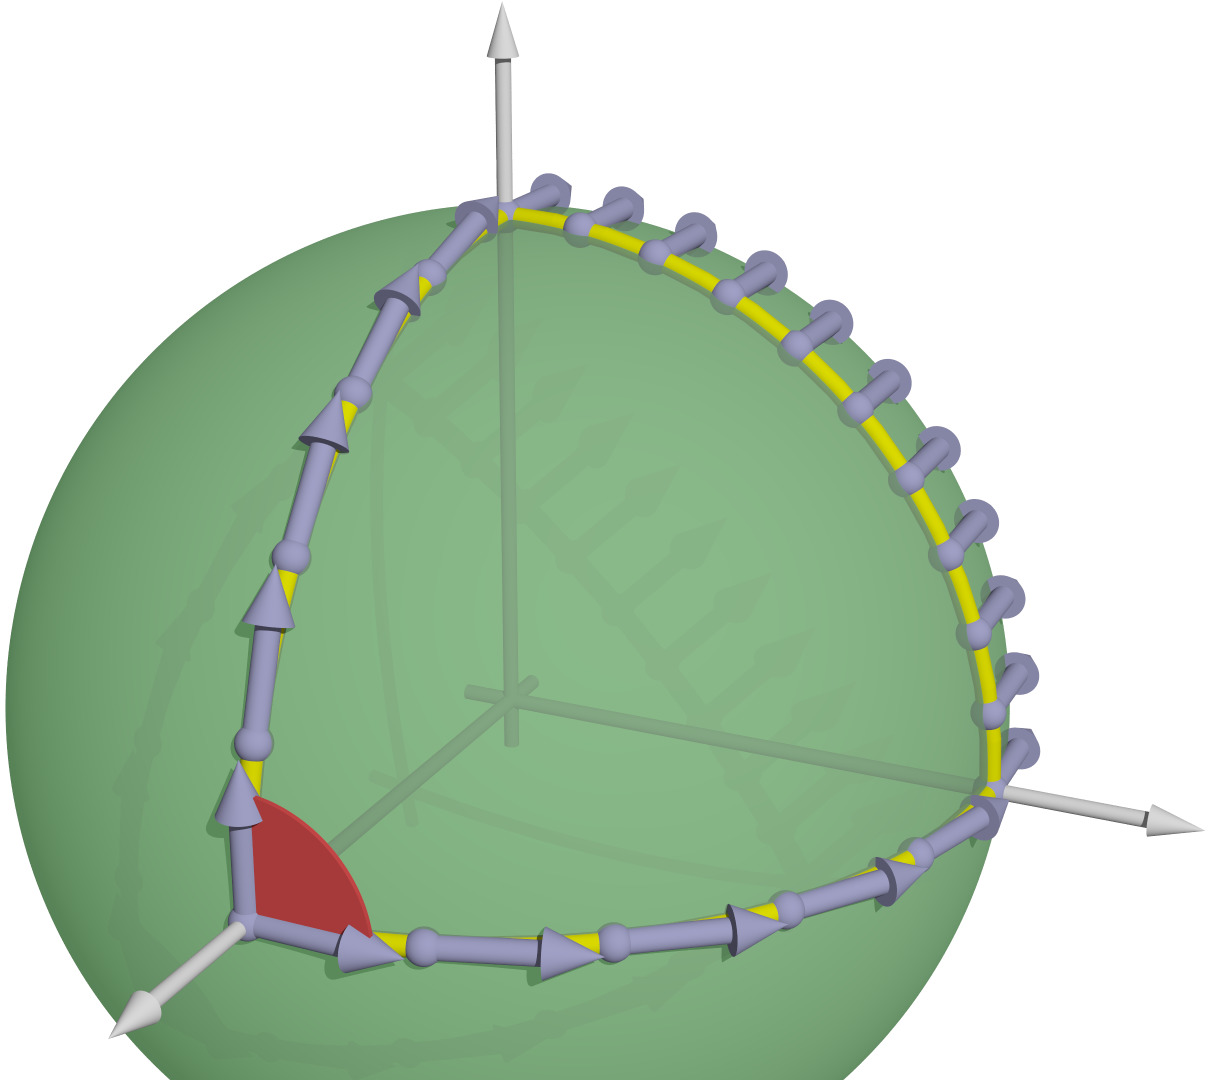
\includegraphics[width=\hsize]{chapters/3d/sphere.jpg}
\caption{Drehung eines Tangentialvektors beim Transport entlang eines
Dreiecks auf der Kugeloberfläche.
Der Flächeninhalt des Dreiecks ist ein Achtel der Kugeloberfläche,
also $4\pi/8=\pi/2$, der Drehwinkel ist $\pi/2$.
\label{skript:kruemmung:transportkugel}}
\end{figure}

Transportiert man einen Vektor in der Ebene mit dem üblichen euklidischen
Koordinatensysteme parallel, dann ändert seine Richtung nicht,
denn die Christoffelsymbole verschwinden alle
(Abbildung~\ref{skript:kruemmung:transportflach}).
Auf einer Kugeloberfläche sieht das ganz anders aus.
Transportiert man einen Vektor tangential an den Äquator zunächst entlang 
des Äquators über einen Winkel von $90^\circ$, dann auf einem Längenkreis
bis zum Nordpol und wieder zurück zum Ausgangspunkt.
Wie in Abbildung~\ref{skript:kruemmung:transportkugel}
sichtbar, dreht sich der Vektor
dabei um $90^\circ$. 
Der Unterschied rührt natürlich daher, dass die Kugeloberfläche gekrümmt
ist.
Offenbar ist die Änderung der Richtung eines Tangentialvektors beim
Paralleltransport entlang eines geschlossenen Weges ein Mass für die
Krümmung einer Fläche.

In diesem Kapitel wollen wir zeigen, wie aus dem Konzept des
Paralleltransportes ein mathematisch wohldefiniertes Mass für die
Krümmung gewonnen werden kann.

\subsection{Krümmungstensor}
Wir möchten Berechnen, wie sich ein Vektor beim Paralleltransport entlang
einer geschlossenen Kurve ändert.
In dieser Form ist das Problem sicher zu kompliziert, die Wahl
einer geschlossenen Kurve beinhaltet viel zu viele Freiheitsgrade.

Zu zwei Tangentialvektoren $u^\mu$ und $v^\mu$ und in einem Punkt
$P$ können wir immer eine
Fläche finden, die aus Geodäten besteht, die alle vom Punkt $P$ ausgehen
und dort eine Richtung haben, die eine Linearkombination der beiden
Tangentialvektoren ist.
Mit diesem Trick können wir das Problem auf eine zweidimensionale
Fläche reduzieren.
Und statt eine beliebige Kurve zuzulassen, können wir uns weiter
auf einen Polygonzug beschränken, bei dem wir den Geodäten folgen,
die als Tangentialrichtung die Richtung der beiden gegebenen
Tangentialvektoren haben.

Wenn wir einen Vektor $A^\mu$ entlang einer solchen Kurve parallel
transportieren, dann aber die Kurve auf einen Punkt zusammenschrumpfen
lassen, dann entsteht im Grenzwert ein Vektor $y^\mu$,
der die Verschiebung des Vektors $A^\mu$ beschreibt.
Dieser Vektor muss linear von $u^\mu$, $v^\mu$ und $A^\mu$ abhängen,
wir erwarten also, dass in jedem Punkt Zahlen
$R^\alpha\mathstrut_{\mu\nu\sigma}$ geben muss, mit denen man
$y^\mu$ berechnen kann:
\[
y^\alpha = R^\alpha\mathstrut_{\mu\nu\sigma}u^\mu v^\nu A^\sigma.
\]

\subsubsection{Wegintegral und Gebietsintegral in der Ebene}
In diesem Abschnitt betrachten wir Funktionen $f(x,y)$ und $g(x,y)$
in der Ebene und ein Teilgebiet $D\subset \mathbb R^2$, welches
von einer Kurve $c\colon [a,b]\to\mathbb R^2\colon t\mapsto c(t)$
berandet wird.
Die beiden Funktionen $f$ und $g$ kann man auch als ein zweidimensionales
Vektorfeld in der Ebenen $\mathbb R^2$ betrachten, jedem Punkt der
Ebene ist ein Vektor 
\[
(x,y)\mapsto \vec{v}(x,y)=\begin{pmatrix}f(x,y)\\g(x,y)\end{pmatrix}
\]
zugeordnet.

\begin{definition}
Das Wegintegral des $\vec v$ entlang der Kurve $c(t)=(x(t),y(t))$ ist
\[
\oint_c (f\,dx + g\,dy)
= 
\int_a^b f(x(t),y(t)) \dot x(t) + g(x(t),y(t)) \dot y(t)\,dt.
\]
\end{definition}

Zu dem gegebenen Gebiet $D$ kann man aber auch für jede beliebige
Funktion $h(x,y)$ das Gebietsintegral bilden.
Wir tun dies im Detail nur für Gebiete deren Rand sich durch zwei
Funktionen $y_1(x)$ und $y_2(x)$ beschreiben lassen, so dass das
Gebiet $D$ durch
\[
D=\{ (x,y) \,|\, y_1(x) \le y \le y_2(x), x_1\le x\le x_2\}
\]
beschrieben werden kann.
Dann definieren wir

\begin{definition}
Das Gebietsintegral von $h(x,y)$ im Gebiet $D$ ist
\[
\int_D h(x,y)\,dx\,dy = \int_{x_1}^{x_2} \int_{y_1(x)}^{y_2(x)} h(x,y)\,dy\,dx
\]
\end{definition}

Lässt sich das Gebiet ausserdem mit zwei Funktion $x_1(y)$ und $x_2(y)$
in der Form
\[
D=\{(x,y)\,|\, x_1(y)\le x\le x_2(y), y_1\le y\le y\le y_2\}
\]
beschreiben, dann kann man das Gebietsintegral auch als
\[
\int_Dh(x,y)\,dx\,dy
=
\int_{y_1}^{y_2}\int_{x_1(y)}^{x_2(y)} h(x,y)\,dx\,dy
\]
schreiben, und die beiden Formeln stimmen überein.

\subsubsection{Der Satz von Green}
Der Satz von Green stellt einen Zusammenhang zwischen einem Wegintegral
und einem Flächenintegral her.

\begin{satz}[Green]
Sind $f$ und $g$ stetig differenzierbare Funktionen im Gebiet $D$, welches
von der Kurve $c$ berandet ist, dann gilt
\[
\oint_c (f\,dx + g\,dy)
=
\int_D \biggl(\frac{\partial g}{\partial x}
   -\frac{\partial f}{\partial y}\biggr)\,dx\,dy
\]
\end{satz}

\begin{proof}[Beweis]
Wir gehen davon aus, dass wir das Gebiet $D$ durch die Kurven $x_1(y)$
und $x_2(y)$ bzw.~$y_1(x)$ und $y_2(x)$ beschreiben können.
Sollte dies nicht möglich sein, muss das Gebiet in Teilgebiet zerlegt
werden, für die dies möglich ist.
Die Wegintegral über die gemeinsamen Teile des Ränder der Teilgebiet 
heben sich weg.

Wir berechnen jetzt die einzelnen Summanden der rechten Seite.
\begin{align*}
\int_D -\frac{\partial f}{\partial y}\,dx\,dy
&=
\int_{x_1}^{x_2}
\int_{y_1(x)}^{y_2(x)} -\frac{\partial f}{\partial y}\,dy \,dx
=
-\int_{x_1}^{x_2} \biggl[f(x,y)\biggr]_{y_1(x)}^{y_2(x)} 
\,dx
\\
&=
\int_{x_1}^{x_2} -f(x,y_2(x))+f(x,y_1(x))\,dx
=
\int_{x_1}^{x_2} f(x,y_1(x))\,dx - \int_{x_1}^{x_2} f(x,y_2(x))\,dx
\\
&=
\int_{x_1}^{x_2} f(x,y_1(x))\,dx + \int_{x_2}^{x_1} f(x,y_2(x))\,dx
\end{align*}
Der erste Term ist das Wegintegral entlang des unteren Randes des
Gebietes $D$ mit der Parametrisierung $x\mapsto(x,y_1(x))$,
der zweite Term is das Wegintegral entlang des oberen Randes des
Gebietes $D$ mit der Parametrisierung $x\mapsto(x,y_2(x))$.
Auf der rechten Seite steht also das Wegintegral 
\[
\int_{x_1}^{x_2}
\int_{y_1(x)}^{y_2(x)} -\frac{\partial f}{\partial y}\,dy \,dx
=
\oint_c f\,dx.
\]
Analog kann man für die partielle Ableitung von $g$ mit der anderen
Beschreibung der Gebietsränder finden
\begin{align*}
\int_D \frac{\partial g}{\partial x}\,dx\,dy
&=
\int_{y_1}^{y_2}
\int_{x_1(y)}^{x_2(y)} \frac{\partial g}{\partial x}\,dx\,dy
=
\int_{y_1}^{y_2} \biggl[g(x,y)\biggr]_{x_1(y)}^{x_2(y)} \,dy
=
\int_{y_1}^{y_2} g(x_2(y),y) - g(x_1(y),y) \,dy
\\
&=
\int_{y_1}^{y_2} g(x_2(y),y) \,dy + \int_{y_2}^{y_1} g(x_1(y),y)\,dy
=
\oint_c g\,dy
\end{align*}
Das letzte Gleichheitszeichen folgt wieder, weil $y\mapsto (x_2(y),y)$ den
rechten Rand von $D$ beschreibt, $y\mapsto (x_1(y),y)$ den linken,
wobei auf dem linken Teil der Parameter von $y=y_2$ zu $y=y_1$
laufen muss.
Addiert man beide Gleichungen erhält man
\[
\int_D \frac{\partial g}{\partial x}-\frac{\partial f}{\partial y}\,dx\,dy
=
\oint_c (f\,dx + g\,dy),
\]
also die Aussage des Satzes von Green.
\end{proof}

\subsubsection{Der Satz von Stokes}
Der Satz von Stokes stellt einen Zusammenhang her zwischen dem Verhalten
eines Vektorfeldes entlang einer geschlossenen Kurve und den Ableitungen
des Vektorfeldes im inneren der Kurve.

Sei also $A_i$ ein Vektorfeld und $x^i(t)$ eine Kurve.
Dann kann man das Kurvenintegral entlang der 

\subsubsection{Der Krümmiunmgstensor}

\subsection{Ricci-Krümmung}

